\subsection*{(a)}
5/5 vision is defined as resolving each optotype with thickness subtended by 1 minute ($ 1/\ang{60} = \ang{0.0166}$) and size subtended by 5 minutes ($ 5/\ang{60} = \ang{0.0833}$):
\begin{equation}
    \begin{split}
        &h = 2d \cdot \tan \left(\frac{\theta}{2}\right) \\
        &\text{Size} = 2 \cdot 5 \cdot \tan(0.0417) = \SI{7.3}{mm} \\
        &\text{Thickness}  = 2 \cdot 5 \cdot \tan(0.0083) = \SI{1.5}{mm}
    \end{split}
\end{equation}

Acuity is distance of test / distance at which the optotype was resolved. The sizes and thickness are calculated similarly to the above.

\begin{table}[h] \centering
    \begin{tabular}{ccccc}
        \toprule
        Row & Acuity & Size (mm) & Thickness (mm) & Letters\\
        \midrule
        1 & 5/50 &72.7 & 14.5 & E \\
        2 & 5/25& 36.4 & 7.3 & FP \\
        3 & 5/17.5&25.5 & 5.1 & TOZ \\
        4 & 5/12.5&18.2 & 3.6 & LPED \\
        5 & 5/10& 14.5 & 2.9 & PECFD \\
        6 & 5/7.5& 10.9 & 2.2 & EDFCZP \\
        7 & 5/6 &8.7 & 1.7 & FELOPZD \\
        8 & 5/5& 7.3 & 1.5 & DEFPOTEC \\
        9 & 5/4& 5.8 & 1.2 & LEFODPCT \\
        \bottomrule
    \end{tabular}
    \caption{Snellen chart based on a 5 meter distance utilising standard letters for each row.}
\end{table}

\subsection*{(b)}
Considering that the farthest John can see is 0.4 m, he is myopic. This is corrected with diverging lenses, which we would expect to be of negative meniscus (concave + convex surface) or biconcave shape. 

We calculate the focal length, $f$, by using the thin lens equation and assuming a distance of 2 cm between the eyes and the glasses:
\begin{equation}\begin{split}
    \frac{1}{f} = \frac{1}{d_o} + \frac{1}{d_i - 0.02} \\
    \frac{1}{f} = \cancelto{0}{\frac{1}{d_o}} - \frac{1}{0.4-0.02} \\
    f = -\SI{0.38}{m}
\end{split}
\end{equation}
From which we may also deduce the lens power: $\frac{1}{f} = -\SI{2.6316}{m^{-1}}$

\begin{figure}[h!]\centering
    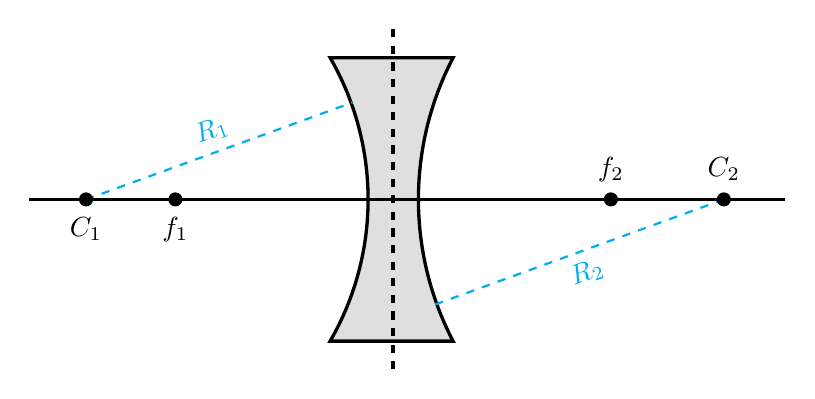
\begin{tikzpicture}[bullet/.style={circle,black,fill,inner sep=1.8pt},
    every label/.append style={black},
    declare function={lensf(\n,\d,\Rone,\Rtwo)=1/(
    (\n-1)*(1/\Rone-1/\Rtwo+(\n-1)*\d/(\n*\Rone*\Rtwo)));
    startangle(\h,\r)=asin(\h/\r);},
    lens/.cd,n/.initial=1.7,R1/.initial=3.6,R2/.initial=-3.9,d/.initial=0.6,
    h/.initial=1.8,alpha/.initial=20]
   %short cut 
   \def\pv#1{\pgfkeysvalueof{/tikz/lens/#1}} 
 
   \draw [fill=lightgray!50, very thick]  
     ({-\pv{d}/2-cos(90-startangle(\pv{h},\pv{R1}))},\pv{h})
     arc[start angle={startangle(\pv{h},\pv{R1})},delta 
     angle={-2*startangle(\pv{h},\pv{R1})},radius=\pv{R1}]
     --++ ({\pv{d}+cos(90-startangle(\pv{h},\pv{R1}))+cos(90+startangle(\pv{h},\pv{R2}))},0)
     arc[start angle={-startangle(\pv{h},\pv{R2})},delta 
     angle={2*startangle(\pv{h},\pv{R2})},radius=\pv{R2}]  
     -- cycle;
    \draw[very thick,dashed] (0,-1.2*\pv{h}) --  (0,1.2*\pv{h});
    \draw[very thick] (-1.2*\pv{R1}-\pv{d}/2,0) -- (-1.2*\pv{R2}+\pv{d}/2,0);
    \draw[cyan,dashed,thick] ({-\pv{d}/2-\pv{R1}},0)   
     node[bullet,label=below:$C_1$]{}
    -- node[sloped,above]{$R_1$} ++ (\pv{alpha}:\pv{R1});
    \path ({-lensf(\pv{n},\pv{d},\pv{R1},\pv{R2})},0) 
     node[bullet,label=below:$f_1$]{};
    \draw[cyan,dashed,thick] ({\pv{d}/2-1*\pv{R2}},0)    
     node[bullet,label=above:$C_2$]{}
    -- node[sloped,below]{$R_2$} ++ (\pv{alpha}:\pv{R2});
    \path ({lensf(\pv{n},\pv{d},-1*\pv{R2},-1*\pv{R1})},0) 
     node[bullet,label=above:$f_2$]{};
  \end{tikzpicture}
  \caption{Representation of lens as biconcave for simplicity's sake}
\end{figure}
Using the lens maker's equation and the following assumptions:
\begin{itemize}
    \item The refractive index of glass/air is 1.5;
    \item Thin lenses, $d \approx 0$;
    \item Lens is biconcave, therefore the radii of curvatuve, $R_1 = -R_2$
\end{itemize}
\begin{equation}
\begin{split}
    \frac{1}{f} = (n-1) \left[
        \frac{1}{R_1} - \frac{1}{R_2} + \frac{(n-1)d}{nR_1R_2}
    \right] \\
    -2.6316 = (1.5-1)(\frac{2}{R}) \\
    R = -\SI{38.00}{cm}
\end{split}
\end{equation}
Finally, reflection only accounts for about 4\% loss in light transmission, so there is little concern about the glass lenses themselves:
\begin{equation}
    \text{Reflectivity} = {\left( \frac{n_2-n_1}{n_2+n_1} \right)}^2 = {\left( \frac{1.5-1}{1.5+1} \right)}^2 = 0.04 = 4\%
\end{equation}